\documentclass[notheorems, aspectratio=149]{beamer}
% aspectratio: 1610, 149, 54, 43(default), 32

\usepackage{bibentry}
% \usepackage[backend=biber,style=ieee, citestyle=authoryear,uniquename=full]{biblatex}
\usepackage{biblatex}
\renewcommand*{\nameyeardelim}{\addcomma\addspace}

\bibliography{refs.bib}

% Input and encoding
\usepackage[utf8]{inputenc}
\usepackage[utf8]{vietnam}
\usepackage{lmodern}

% Math packages
\usepackage{amsmath,amssymb,amsthm}
\usepackage{mathtools}
\usepackage{physics} % For better physics notation

% Common math symbols
\newcommand{\N}{\mathbb{N}}
\newcommand{\Z}{\mathbb{Z}}
\newcommand{\Q}{\mathbb{Q}}
\newcommand{\R}{\mathbb{R}}
\newcommand{\C}{\mathbb{C}}
\newcommand{\F}{\mathbb{F}}

% Graphics and colors
\usepackage{graphicx}
\usepackage[dvipsnames]{xcolor}
\usepackage{tikz,tikz-3dplot}
\usepackage{pgfplots}
\pgfplotsset{compat=1.18}

% TikZ libraries
\usetikzlibrary{
    calc,trees,positioning,arrows,chains,shapes.geometric,
    decorations.pathreplacing,decorations.pathmorphing,shapes,
    matrix,shapes.symbols,fit,arrows.meta,backgrounds,
    decorations.markings,patterns,3d
}

% Tables and captions
\usepackage{booktabs}
\usepackage{array}
\usepackage{caption}
\usepackage{subcaption}
\setbeamertemplate{caption}[numbered]

% Text formatting and algorithms
\usepackage{ulem}
\usepackage{algorithm}
\usepackage{algorithmic}
% \usepackage{algpseudocode}
\usepackage{listings}
% \usepackage{enumitem}

% Hyperlinks
\usepackage{hyperref}
\hypersetup{
    colorlinks=true,
    linkcolor=blue,
    filecolor=magenta,
    urlcolor=cyan,
    citecolor=green
}

% =============================================================================
% COLOR SCHEME
% =============================================================================

\definecolor{primaryblue}{HTML}{0065BD}
\definecolor{secondaryblue}{HTML}{4A90E2}
\definecolor{accentorange}{HTML}{FF6B35}
\definecolor{darkgray}{HTML}{2C3E50}
\definecolor{lightgray}{HTML}{ECF0F1}
\definecolor{successgreen}{HTML}{27AE60}
\definecolor{warningred}{HTML}{E74C3C}

% =============================================================================
% BEAMER THEME CONFIGURATION
% =============================================================================

\mode<presentation>{
    \usetheme{default}
    \useoutertheme{infolines}
    \useinnertheme{circles}
    \setbeamercovered{transparent}
    \setbeamertemplate{theorems}[numbered]
    \setbeamertemplate{navigation symbols}{}
}

% Custom color theme
\setbeamercolor{structure}{fg=primaryblue}
\setbeamercolor{frametitle}{bg=primaryblue,fg=white}
\setbeamercolor{title}{fg=primaryblue}
\setbeamercolor{subtitle}{fg=darkgray}
\setbeamercolor{author}{fg=darkgray}
\setbeamercolor{block title}{bg=secondaryblue,fg=white}
\setbeamercolor{block body}{bg=lightgray,fg=darkgray}
\setbeamercolor{block title alerted}{bg=warningred,fg=white}
\setbeamercolor{block body alerted}{bg=warningred!10,fg=darkgray}
\setbeamercolor{block title example}{bg=successgreen,fg=white}
\setbeamercolor{block body example}{bg=successgreen!10,fg=darkgray}

% =============================================================================
% CUSTOM FRAME ENVIRONMENTS
% =============================================================================

\usepackage{framed}
\pgfmathsetseed{1}

% Define layers for parchment effect
\pgfdeclarelayer{background}
\pgfsetlayers{background,main}

% Parchment styles
\tikzset{
    normal border/.style={
        primaryblue!40!black!10, decorate,
        decoration={random steps, segment length=2.5cm, amplitude=.7mm}
    },
    torn border/.style={
        primaryblue!40!black!5, decorate,
        decoration={random steps, segment length=.5cm, amplitude=1.7mm}
    }
}

% Parchment frame macros
\def\parchmentframe#1{
    \tikz{
        \node[inner sep=2em] (A) {#1};
        \begin{pgfonlayer}{background}
            \fill[normal border] 
                (A.south east) -- (A.south west) -- 
                (A.north west) -- (A.north east) -- cycle;
        \end{pgfonlayer}
    }
}

\def\parchmentframetop#1{
    \tikz{
        \node[inner sep=2em] (A) {#1};
        \begin{pgfonlayer}{background}    
            \fill[normal border]
                (A.south east) -- (A.south west) -- 
                (A.north west) -- (A.north east) -- cycle;
            \fill[torn border]
                ($(A.south east)-(0,.2)$) -- ($(A.south west)-(0,.2)$) -- 
                ($(A.south west)+(0,.2)$) -- ($(A.south east)+(0,.2)$) -- cycle;
        \end{pgfonlayer}
    }
}

\def\parchmentframebottom#1{
    \tikz{
        \node[inner sep=2em] (A) {#1};
        \begin{pgfonlayer}{background}   
            \fill[normal border]
                (A.south east) -- (A.south west) -- 
                (A.north west) -- (A.north east) -- cycle;
            \fill[torn border]
                ($(A.north east)-(0,.2)$) -- ($(A.north west)-(0,.2)$) -- 
                ($(A.north west)+(0,.2)$) -- ($(A.north east)+(0,.2)$) -- cycle;
        \end{pgfonlayer}
    }
}

\def\parchmentframemiddle#1{
    \tikz{
        \node[inner sep=2em] (A) {#1};
        \begin{pgfonlayer}{background}   
            \fill[normal border]
                (A.south east) -- (A.south west) -- 
                (A.north west) -- (A.north east) -- cycle;
            \fill[torn border]
                ($(A.south east)-(0,.2)$) -- ($(A.south west)-(0,.2)$) -- 
                ($(A.south west)+(0,.2)$) -- ($(A.south east)+(0,.2)$) -- cycle;
            \fill[torn border]
                ($(A.north east)-(0,.2)$) -- ($(A.north west)-(0,.2)$) -- 
                ($(A.north west)+(0,.2)$) -- ($(A.north east)+(0,.2)$) -- cycle;
        \end{pgfonlayer}
    }
}

\newenvironment{parchment}[1][Example]{%
    \def\FrameCommand{\parchmentframe}%
    \def\FirstFrameCommand{\parchmentframetop}%
    \def\LastFrameCommand{\parchmentframebottom}%
    \def\MidFrameCommand{\parchmentframemiddle}%
    \vskip\baselineskip
    \MakeFramed{\FrameRestore}
    \noindent\tikz\node[inner sep=1ex, draw=white, fill=primaryblue!30, 
        anchor=west, overlay] at (0em, 2em) {\sffamily#1};\par
}{%
    \endMakeFramed
}

% =============================================================================
% TITLE PAGE CUSTOMIZATION
% =============================================================================

\makeatletter
\newcommand\titlegraphicii[1]{\def\inserttitlegraphicii{#1}}
\titlegraphicii{}

\setbeamertemplate{title page}{
    {\usebeamercolor[fg]{titlegraphic}\inserttitlegraphic\hfill\inserttitlegraphicii\par}
    \begin{centering}
        \vskip1em
        \begin{beamercolorbox}[sep=8pt,center]{title}
            \usebeamerfont{title}\inserttitle\par%
            \ifx\insertsubtitle\@empty%
            \else%
                \vskip0.5em%
                {\usebeamerfont{subtitle}\usebeamercolor[fg]{subtitle}\insertsubtitle\par}%
            \fi%     
        \end{beamercolorbox}%
        \vskip1em
        \begin{beamercolorbox}[sep=8pt,center]{author}
            \usebeamerfont{author}\insertauthor
        \end{beamercolorbox}
        \vskip1em
        \begin{beamercolorbox}[sep=8pt,center]{institute}
            \usebeamerfont{institute}\insertinstitute
        \end{beamercolorbox}
        \vskip1em
        \begin{beamercolorbox}[sep=8pt,center]{date}
            \usebeamerfont{date}\insertdate
        \end{beamercolorbox}
    \end{centering}
    \vfill
}

% =============================================================================
% HEADER AND FOOTER
% =============================================================================

\setbeamertemplate{frametitle}{%
    \nointerlineskip%
    \begin{beamercolorbox}[wd=\paperwidth,ht=2.5ex,dp=1.125ex]{frametitle}
        \hspace*{1em}\insertframetitle%
        \ifx\insertframesubtitle\@empty%
        \else%
            \par\hspace*{1em}{\usebeamerfont{framesubtitle}\insertframesubtitle}%
        \fi%
    \end{beamercolorbox}%
}

\setbeamertemplate{footline}{
    \leavevmode%
    \hbox{%
        \begin{beamercolorbox}[wd=.25\paperwidth,ht=2.25ex,dp=1ex,center]{author in head/foot}%
            \usebeamerfont{author in head/foot}\insertpresenter
        \end{beamercolorbox}%
        \begin{beamercolorbox}[wd=.5\paperwidth,ht=2.25ex,dp=1ex,center]{title in head/foot}%
            \usebeamerfont{title in head/foot}\insertshorttitle
        \end{beamercolorbox}%
        \begin{beamercolorbox}[wd=.25\paperwidth,ht=2.25ex,dp=1ex,center]{date in head/foot}%
            \insertframenumber{} / \inserttotalframenumber\hspace*{1ex}
        \end{beamercolorbox}%
    }%
    \vskip0pt%
}

% =============================================================================
% SECTION PAGES
% =============================================================================

\setbeamertemplate{section page}{
    \begin{centering}
        \vskip2em
        \begin{beamercolorbox}[sep=12pt,center]{part title}
            \usebeamerfont{section title}\insertsection\par
        \end{beamercolorbox}
        \vskip2em
    \end{centering}
}

% \AtBeginSection[]{
%     \begin{frame}[plain,noframenumbering]
%         \sectionpage
%         \tableofcontents[currentsection,hideothersubsections]
%     \end{frame}
% }

% =============================================================================
% THEOREM ENVIRONMENTS
% =============================================================================

\usepackage{thmtools}
\usepackage[framemethod=TikZ]{mdframed}
\mdfsetup{skipabove=1em,skipbelow=1em}

% Theorem styles
\declaretheoremstyle[
    headfont=\bfseries\color{successgreen!70!black},
    bodyfont=\normalfont,
    % mdframed={
    %     linewidth=2pt,
    %     rightline=false, topline=false, bottomline=false,
    %     linecolor=successgreen, backgroundcolor=successgreen!5,
    % }
]{thmwhitebox}

\declaretheoremstyle[
    headfont=\bfseries\color{successgreen!70!black},
    bodyfont=\normalfont,
    mdframed={
        linewidth=2pt,
        rightline=false, topline=false, bottomline=false,
        linecolor=successgreen, backgroundcolor=successgreen!5,
    }
]{thmgreenbox}

\declaretheoremstyle[
    headfont=\bfseries\color{primaryblue!70!black},
    bodyfont=\normalfont,
    mdframed={
        linewidth=2pt,
        rightline=false, topline=false, bottomline=false,
        linecolor=primaryblue, backgroundcolor=primaryblue!5,
    }
]{thmbluebox}

\declaretheoremstyle[
    headfont=\bfseries\color{primaryblue!70!black},
    bodyfont=\normalfont,
    mdframed={
        linewidth=2pt,
        rightline=false, topline=false, bottomline=false,
        linecolor=primaryblue
    }
]{thmblueline}

\declaretheoremstyle[
    headfont=\bfseries\color{warningred!70!black},
    bodyfont=\normalfont,
    mdframed={
        linewidth=2pt,
        rightline=false, topline=false, bottomline=false,
        linecolor=warningred, backgroundcolor=warningred!5,
    }
]{thmredbox}

\declaretheoremstyle[
    headfont=\bfseries\color{accentorange!70!black},
    bodyfont=\normalfont,
    mdframed={
        linewidth=2pt,
        rightline=false, topline=false, bottomline=false,
        linecolor=accentorange, backgroundcolor=accentorange!5,
    }
]{thmorangebox}

\declaretheoremstyle[
    headfont=\bfseries\color{warningred!70!black},
    bodyfont=\normalfont,
    numbered=no,
    mdframed={
        linewidth=2pt,
        rightline=false, topline=false, bottomline=false,
        linecolor=warningred, backgroundcolor=warningred!1,
    },
    qed=\qedsymbol
]{thmproofbox}

% Define theorem environments
\declaretheorem[style=thmwhitebox, name=Bài toán]{problem}
\declaretheorem[style=thmwhitebox, name=Định nghĩa]{definition}
\declaretheorem[style=thmwhitebox, name=Ví dụ]{example}
\declaretheorem[style=thmwhitebox, name=Nhận xét]{remark}
\declaretheorem[style=thmwhitebox, name=Định lý]{theorem}
\declaretheorem[style=thmwhitebox, name=Bổ đề]{lemma}
\declaretheorem[style=thmwhitebox, name=Mệnh đề]{proposition}
\declaretheorem[style=thmwhitebox, name=Hệ quả]{corollary}
\declaretheorem[style=thmwhitebox, name=Khẳng định]{claim}
\declaretheorem[style=thmwhitebox, name=Chú ý]{mynote}
\declaretheorem[style=thmwhitebox, name=Câu hỏi]{question}

% Proof environment
\declaretheorem[style=thmproofbox, name=Proof]{replacementproof}
\renewenvironment{proof}[1][\proofname]{\vspace{-10pt}\begin{replacementproof}}{\end{replacementproof}}

% =============================================================================
% CODE LISTINGS
% =============================================================================

\lstdefinestyle{moderncode}{
    basicstyle=\ttfamily\footnotesize,
    keywordstyle=\color{primaryblue}\bfseries,
    commentstyle=\color{successgreen}\itshape,
    stringstyle=\color{warningred},
    numberstyle=\tiny\color{darkgray},
    breaklines=true,
    breakatwhitespace=false,
    showspaces=false,
    showstringspaces=false,
    showtabs=false,
    tabsize=2,
    numbers=left,
    frame=leftline,
    frameround=fttt,
    framexleftmargin=2em,
    xleftmargin=2em,
    backgroundcolor=\color{lightgray!30},
    rulecolor=\color{primaryblue},
}

\lstset{style=moderncode}

% =============================================================================
% FLOWCHART SETTINGS
% =============================================================================

\tikzset{
    >=stealth',
    punktchain/.style={
        rectangle, 
        rounded corners=3pt, 
        draw=primaryblue, 
        very thick,
        fill=primaryblue!10,
        text width=6em,
        minimum height=2.5em, 
        text centered, 
        on chain
    },
    largepunktchain/.style={
        rectangle,
        rounded corners=3pt,
        draw=primaryblue, 
        very thick,
        fill=primaryblue!10,
        text width=10em,
        minimum height=2.5em,
        text centered,
        on chain
    },
    decision/.style={
        diamond,
        draw=warningred,
        very thick,
        fill=warningred!10,
        text width=4em,
        minimum height=2em,
        text centered,
        on chain
    },
    line/.style={draw, thick, ->},
    every join/.style={->, thick, shorten >=1pt},
    font={\fontsize{10pt}{12}\selectfont},
}

% =============================================================================
% UTILITY COMMANDS
% =============================================================================

% Highlighting
\newcommand{\highlight}[1]{\colorbox{accentorange!20}{#1}}
\renewcommand{\alert}[1]{\textcolor{warningred}{\textbf{#1}}}
\newcommand{\emphasis}[1]{\textcolor{primaryblue}{\textbf{#1}}}

% Math operators (check if already defined)
% \providecommand{\rank}{}
% \renewcommand{\rank}{\operatorname{rank}}
% \providecommand{\trace}{}
% \renewcommand{\trace}{\operatorname{tr}}
% \DeclareMathOperator{\diag}{diag}
% \providecommand{\span}{}
% \renewcommand{\span}{\operatorname{span}}
% \DeclareMathOperator{\dimension}{dim}
% \DeclareMathOperator{\ker}{ker}
% \DeclareMathOperator{\im}{im}


% =============================================================================
% CUSTOM TITLE PAGE
% =============================================================================
% Define custom commands for title page information
\newcommand{\university}[1]{\def\insertuniversity{#1}}
\newcommand{\school}[1]{\def\insertschool{#1}}
\newcommand{\faculty}[1]{\def\insertfaculty{#1}}
\newcommand{\department}[1]{\def\insertdepartment{#1}}
\newcommand{\presenter}[1]{\def\insertpresenter{#1}}
\newcommand{\president}[1]{\def\insertpresident{#1}}
\newcommand{\examinerone}[1]{\def\insertexaminerone{#1}}
\newcommand{\examinertwo}[1]{\def\insertexaminertwo{#1}}
\newcommand{\examinerthree}[1]{\def\insertexaminerthree{#1}}
\newcommand{\examinerfour}[1]{\def\insertexaminerfour{#1}}
\newcommand{\supervisorone}[1]{\def\insertsupervisorone{#1}}
\newcommand{\supervisortwo}[1]{\def\insertsupervisortwo{#1}}

\makeatletter
\setbeamertemplate{title page}{
    % \vbox{}
    \vfill
    \begingroup
        \centering
        % School name at top
        \begin{beamercolorbox}[sep=8pt,center]{institute}
            \usebeamerfont{institute}\large\textbf{\MakeUppercase\insertuniversity}\\
            \usebeamerfont{institute}\normalsize\MakeUppercase\insertschool\\
            \usebeamerfont{institute}\normalsize\MakeUppercase\insertfaculty
            % \usebeamerfont{institute}\normalsize\MakeUppercase\insertdepartment
        \end{beamercolorbox}\par
        
        \vskip1.em\par
        
        % Title
        \begin{beamercolorbox}[sep=8pt,center]{title}
            \usebeamerfont{title}\Large\textbf{\MakeUppercase\inserttitle}\par%
            \ifx\insertsubtitle\@empty%
            \else%
                \vskip0.5em%
                {\usebeamerfont{subtitle}\large\insertsubtitle\par}%
            \fi%     
        \end{beamercolorbox}\par
        
        \vskip1.em\par
        
        % Presenter
        \begin{beamercolorbox}[sep=8pt,center]{author}
            \usebeamerfont{author}
            % \begin{tabular}{@{}p{.35\textwidth}@{\hspace{3pt}}p{.5\textwidth}@{}}
            %     \textbf{Presenter:} \insertpresenter & \textbf{Supervisor 1:} \insertsupervisorone \\
            %     & \textbf{Supervisor 2:} \insertsupervisortwo \\
            % \end{tabular}
            % \begin{center}
            %     \textbf{Học viên cao học:} \insertpresenter \\ 
            %     \textbf{Người hướng dẫn khoa học:} \insertsupervisorone
            % \end{center}
            \begin{center}
                \textbf{}\insertpresenter \\ 
                % \textbf{Người hướng dẫn khoa học:} \insertsupervisorone
            \end{center}
        \end{beamercolorbox}
        
        \vskip1em\par
        
        % Date
        \begin{beamercolorbox}[sep=8pt,center]{date}
            \usebeamerfont{date}\insertdate
        \end{beamercolorbox}\par
        
    \endgroup
    \vfill
}
\makeatother

% Define colors
\definecolor{shap1}{RGB}{0,114,178}
\definecolor{shap2}{RGB}{213,94,0}
\definecolor{shap3}{RGB}{0,158,115}
\definecolor{shap4}{RGB}{204,121,167}

\title{GIÁ TRỊ SHAP TRONG HỌC MÁY GIẢI THÍCH}
\subtitle{SEMINAR BỘ MÔN KHOA HỌC MÁY TÍNH}


\university{ĐẠI HỌC QUỐC GIA THÀNH PHỐ HỒ CHÍ MINH}
% \university{VIETNAM NATIONAL UNIVERSITY, HO CHI MINH CITY}
\school{TRƯỜNG ĐẠI HỌC KHOA HỌC TỰ NHIÊN}
% \school{UNIVERSITY OF SCIENCE}
% \faculty{KHOA TOÁN - TIN HỌC}
\faculty{KHOA CÔNG NGHỆ THÔNG TIN}
% \faculty{FACULTY OF MATHEMATICS AND COMPUTER SCIENCE}
% \faculty{FACULTY OF INFORMATION TECHNOLOGY}
\presenter{Lê Nhựt Nam}
% \president{Dr. President Name}
% \examinerone{Dr. Examiner One}
% \examinertwo{Dr. Examiner Two}
% \examinerthree{Dr. Examiner Three}
% \examinerfour{Dr. Examiner Four}
% \supervisorone{PGS. TS. Võ Sĩ Trọng Long}
% \supervisortwo{Dr. Co-Supervisor Name}

\begin{document}

\begin{frame}[plain]
    \titlepage{}
\end{frame}

\begin{frame}{Nội dung trình bày}
    \tableofcontents
\end{frame}


\section{Giới thiệu chung}

\begin{frame}{SHAP là gì?}
\textbf{SHAP (SHapley Additive exPlanations)} là một phương pháp tiếp cận dựa trên lý thuyết trò chơi để giải thích kết quả đầu ra cho bất kỳ mô hình học máy nào.

\vspace{0.5cm}
\begin{itemize}
    \item Được công bố bởi Lundberg và Lee vào năm 2017.
    \item Dựa trên giá trị Shapley từ lý thuyết trò chơi hợp tác (cooperative game theory).
    \item Cung cấp khả năng diễn giải \textbf{cục bộ} cho các dự đoán của mô hình.
    \item Trả lời câu hỏi \textbf{``Tại sao?''} trong khi mô hình trả lời \textbf{``Bao nhiêu?''}
\end{itemize}

\vspace{0.3cm}
\begin{alertblock}{Điểm then chốt của SHAP}
SHAP định lượng sự đóng góp của mỗi đặc trưng vào một dự đoán cụ thể.
\end{alertblock}
\end{frame}

\begin{frame}{SHAP trong ngữ cảnh Học Máy}
\begin{columns}
\column{0.5\textwidth}
\textbf{Ánh xạ từ Lý thuyết Trò chơi:}
\begin{itemize}
    \item \textbf{Trò chơi (Game)}: Tái tạo kết quả đầu ra của mô hình
    \item \textbf{Người chơi (Player)}: Các đặc trưng trong mô hình
    \item \textbf{Phần thưởng (Reward)}: Giá trị dự đoán
    \item \textbf{Liên minh (Coalition)}: Tập con các đặc trưng
\end{itemize}

\column{0.5\textwidth}
\textbf{Tính chất chính:}
\begin{itemize}
    \item \textbf{Cục bộ (Local)}: Một quan sát = Một trò chơi
    \item \textbf{Cộng tính (Additive)}: Giá trị SHAP tổng bằng chênh lệch dự đoán
    \item \textbf{Công bằng (Fair)}: Thỏa mãn các tiên đề Shapley
    \item \textbf{Tổng quát (Universal)}: Hoạt động với mọi mô hình
\end{itemize}
\end{columns}

\vspace{0.5cm}
\begin{exampleblock}{Ví dụ}
Mô hình dự đoán thu nhập dựa trên: Tuổi (Age), Giới tính (Sex), Nghề nghiệp (Occupation).
\end{exampleblock}
\end{frame}

\section{Cơ sở toán học cho giá trị SHAP}

\begin{frame}{Ký hiệu toán học}
\begin{block}{Ký hiệu}
\begin{itemize}
    \item $\mathcal{F} = \{1, 2, ..., F\}$: Tập hợp tất cả các đặc trưng
    \item $S \subseteq \mathcal{F}$: Một liên minh (tập con) các đặc trưng
    \item $f_S(x_S)$: Mô hình được huấn luyện chỉ với các đặc trưng trong $S$
    \item $x_i$: Giá trị của đặc trưng $i$ cho quan sát $x$
    \item $\phi_i$: Giá trị SHAP cho đặc trưng $i$
\end{itemize}
\end{block}
\end{frame}

\begin{frame}{Vấn đề trung tâm}
\begin{alertblock}{Vấn đề trung tâm}
Đặc trưng $i$ đóng góp bao nhiêu vào dự đoán $f(x)$ so với dự đoán cơ sở $f_\emptyset$?
\end{alertblock}

\begin{equation}
\sum_{i=1}^{F} \phi_i = f(x) - f_\emptyset
\end{equation}
\end{frame}

\begin{frame}{Tập lũy thừa của các đặc trưng}
\begin{block}{Định nghĩa}
Tập lũy thừa $\mathcal{P}(\mathcal{F})$ (powerset) chứa tất cả các tập con có thể của các đặc trưng
\end{block}
\end{frame}

\begin{frame}{Tập lũy thừa của các đặc trưng}
\begin{columns}
\column{0.5\textwidth}
\textbf{Ví dụ với 3 đặc trưng:}\\
$\mathcal{F} = \{\text{Tuổi, Giới tính, Nghề nghiệp}\}$

\vspace{0.3cm}
Tập lũy thừa có $2^F = 2^3 = 8$ phần tử:
\begin{enumerate}
    \item $\emptyset$ (không đặc trưng)
    \item $\{\text{Tuổi}\}$
    \item $\{\text{Giới tính}\}$
    \item $\{\text{Nghề nghiệp}\}$
    \item $\{\text{Tuổi, Giới tính}\}$
    \item $\{\text{Tuổi, Nghề nghiệp}\}$
    \item $\{\text{Giới tính, Nghề nghiệp}\}$
    \item $\{\text{Tuổi, Giới tính, Nghề nghiệp}\}$
\end{enumerate}

\column{0.5\textwidth}
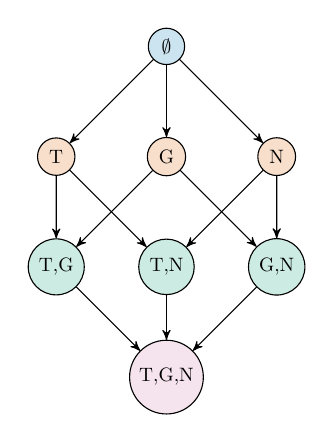
\begin{tikzpicture}[scale=0.7, every node/.style={scale=0.7}]
\node[circle,draw,fill=shap1!20] (empty) at (0,4) {$\emptyset$};
\node[circle,draw,fill=shap2!20] (a) at (-2,2) {T};
\node[circle,draw,fill=shap2!20] (g) at (0,2) {G};
\node[circle,draw,fill=shap2!20] (j) at (2,2) {N};
\node[circle,draw,fill=shap3!20] (ag) at (-2,0) {T,G};
\node[circle,draw,fill=shap3!20] (aj) at (0,0) {T,N};
\node[circle,draw,fill=shap3!20] (gj) at (2,0) {G,N};
\node[circle,draw,fill=shap4!20] (agj) at (0,-2) {T,G,N};

\draw[->] (empty) -- (a);
\draw[->] (empty) -- (g);
\draw[->] (empty) -- (j);
\draw[->] (a) -- (ag);
\draw[->] (a) -- (aj);
\draw[->] (g) -- (ag);
\draw[->] (g) -- (gj);
\draw[->] (j) -- (aj);
\draw[->] (j) -- (gj);
\draw[->] (ag) -- (agj);
\draw[->] (aj) -- (agj);
\draw[->] (gj) -- (agj);
\end{tikzpicture}
\end{columns}
\end{frame}

\section{Đóng góp biên}

\begin{frame}{Định nghĩa của Đóng góp Biên}
\begin{block}{Định nghĩa}
Đóng góp biên của đặc trưng $i$ vào liên minh $S$ (trong đó $i \notin S$):
\begin{equation}
\Delta_i(S) = f_{S \cup \{i\}}(x_{S \cup \{i\}}) - f_S(x_S)
\end{equation}
\end{block}

\begin{exampleblock}{Ví dụ: Thêm Tuổi vào các Liên minh khác nhau}
\begin{itemize}
    \item $\Delta_{\text{Tuổi}}(\emptyset) = f_{\{\text{Tuổi}\}}(x) - f_\emptyset = 40k - 50k = -10k$
    \item $\Delta_{\text{Tuổi}}(\{\text{Giới tính}\}) = f_{\{\text{Tuổi,Giới tính}\}}(x) - f_{\{\text{Giới tính}\}} = 36k - 45k = -9k$
    \item $\Delta_{\text{Tuổi}}(\{\text{Nghề nghiệp}\}) = f_{\{\text{Tuổi,Nghề nghiệp}\}}(x) - f_{\{\text{Nghề nghiệp}\}} = 75k - 90k = -15k$
    \item $\Delta_{\text{Tuổi}}(\{\text{Giới tính,Nghề nghiệp}\}) = f_{\text{Tất cả}}(x) - f_{\{\text{Giới tính,Nghề nghiệp}\}} = 83k - 92k = -9k$
\end{itemize}
\end{exampleblock}
\end{frame}

\begin{frame}{Trực quan hóa Đóng góp biên}
\begin{center}
\begin{tikzpicture}[scale=1]
\tikzstyle{model} = [rectangle, draw, fill=blue!20, text width=3cm, text centered, minimum height=0.8cm]
\tikzstyle{contribution} = [draw, ->, thick, red!70]

% Models
\node[model] (empty) at (0,6) {$\emptyset$: 50k};
\node[model] (age) at (-3,4) {Tuổi: 40k};
\node[model] (gender) at (0,4) {Giới tính: 45k};
\node[model] (job) at (3,4) {Nghề nghiệp: 90k};
\node[model] (age_gender) at (-3,2) {Tuổi,Giới tính: 36k};
\node[model] (age_job) at (0,2) {Tuổi,Nghề: 75k};
\node[model] (gender_job) at (3,2) {Giới tính,Nghề: 92k};
\node[model] (all) at (0,0) {Tất cả: 83k};

% Age contributions (in red)
\draw[contribution] (empty) -- node[left] {-10k} (age);
\draw[contribution] (gender) -- node[left] {-9k} (age_gender);
\draw[contribution] (job) -- node[right] {-15k} (age_job);
\draw[contribution] (gender_job) -- node[right] {-9k} (all);

% Other edges (in gray)
\draw[gray] (empty) -- (gender);
\draw[gray] (empty) -- (job);
\draw[gray] (age) -- (age_gender);
\draw[gray] (age) -- (age_job);
\draw[gray] (gender) -- (gender_job);
\draw[gray] (job) -- (gender_job);
\draw[gray] (age_gender) -- (all);
\draw[gray] (age_job) -- (all);
\end{tikzpicture}
\end{center}

% \textcolor{red}{Mũi tên đỏ}: Đóng góp biên của đặc trưng Tuổi
\end{frame}

\section{Tính toán trọng số}

\begin{frame}{Công thức Trọng số Shapley}
\begin{block}{Trọng số cho Đóng góp biên}
Trọng số cho đóng góp biên của đặc trưng $i$ vào liên minh $S$ có kích thước $|S|$ được cho bởi:
\begin{equation}
w(S) = \frac{|S|!(F-|S|-1)!}{F!}.
\end{equation}
\end{block}

\begin{alertblock}{Ý nghĩa}
\begin{itemize}
    \item Trọng số đảm bảo \textbf{tầm quan trọng bằng nhau} cho mọi kích thước liên minh.
    \item Tổng trọng số cho tất cả liên minh kích thước $s$ bằng $\dfrac{1}{F}$.
    \item Thỏa mãn các tiên đề \textbf{hiệu quả} và \textbf{đối xứng}.
\end{itemize}
\end{alertblock}
\end{frame}

\begin{frame}{Công thức Trọng số Shapley}
\begin{block}{Trọng số cho Đóng góp biên}
Trọng số cho đóng góp biên của đặc trưng $i$ vào liên minh $S$ có kích thước $|S|$:
\begin{equation}
w(S) = \dfrac{|S|!(F-|S|-1)!}{F!}
\end{equation}
\end{block}

\begin{exampleblock}{Ví dụ: Trọng số cho Đặc trưng Tuổi ($F=3$)}
\begin{itemize}
    \item $w(\emptyset) = \dfrac{0! \cdot 2!}{3!} = \dfrac{2}{6} = \dfrac{1}{3}$
    \item $w(\{\text{Giới tính}\}) = w(\{\text{Nghề nghiệp}\}) = \dfrac{1! \cdot 1!}{3!} = \dfrac{1}{6}$
    \item $w(\{\text{Giới tính, Nghề nghiệp}\}) = \dfrac{2! \cdot 0!}{3!} = \dfrac{2}{6} = \dfrac{1}{3}$
\end{itemize}
\end{exampleblock}
\end{frame}

\begin{frame}{Cách tính Trọng số Thay thế}
\begin{block}{Số Cạnh mỗi Cấp}
Với mô hình có $f$ đặc trưng, tổng số đóng góp biên là:
\begin{equation}
\text{Số cạnh tại cấp } f = f \cdot \binom{F}{f}
\end{equation}
\end{block}
\end{frame}

\begin{frame}{Cách tính Trọng số Thay thế}
\begin{columns}
\column{0.5\textwidth}
\textbf{Ví dụ Tính toán ($F=3$):}
\begin{itemize}
    \item Cấp 1: $1 \cdot \binom{3}{1} = 3$ cạnh
    \item Cấp 2: $2 \cdot \binom{3}{2} = 6$ cạnh
    \item Cấp 3: $3 \cdot \binom{3}{3} = 3$ cạnh
\end{itemize}

\vspace{0.3cm}
\textbf{Trọng số:}
\begin{itemize}
    \item Cấp 1: $\frac{1}{3}$ mỗi cạnh
    \item Cấp 2: $\frac{1}{6}$ mỗi cạnh
    \item Cấp 3: $\frac{1}{3}$ mỗi cạnh
\end{itemize}

\column{0.5\textwidth}
\begin{tikzpicture}[scale=0.7]
\node at (0,4) {Cấp 0};
\node at (0,2.5) {Cấp 1 (3 cạnh)};
\node at (0,1) {Cấp 2 (6 cạnh)};
\node at (0,-0.5) {Cấp 3 (3 cạnh)};

\draw[thick,->] (-1,3.5) -- (-1,2.8) node[midway,left] {$\frac{1}{3}$};
\draw[thick,->] (0,3.5) -- (0,2.8);
\draw[thick,->] (1,3.5) -- (1,2.8);

\draw[thick,->] (-2,2.2) -- (-2,1.5) node[midway,left] {$\frac{1}{6}$};
\draw[thick,->] (-1.2,2.2) -- (-1.2,1.5);
\draw[thick,->] (-0.4,2.2) -- (-0.4,1.5);
\draw[thick,->] (0.4,2.2) -- (0.4,1.5);
\draw[thick,->] (1.2,2.2) -- (1.2,1.5);
\draw[thick,->] (2,2.2) -- (2,1.5);

\draw[thick,->] (-1,0.7) -- (-1,0) node[midway,left] {$\frac{1}{3}$};
\draw[thick,->] (0,0.7) -- (0,0);
\draw[thick,->] (1,0.7) -- (1,0);
\end{tikzpicture}
\end{columns}
\end{frame}

\section{Biểu thức SHAP đầy đủ}

\begin{frame}{Công thức Giá trị SHAP}
\begin{block}{Định nghĩa}
Giá trị SHAP cho đặc trưng $i$ là:
\begin{equation}
\phi_i(x) = \sum_{S \subseteq \mathcal{F} \setminus \{i\}} \frac{|S|!(F-|S|-1)!}{F!} \cdot \left[f_{S \cup \{i\}}(x_{S \cup \{i\}}) - f_S(x_S)\right]
\end{equation}
\end{block}

\begin{alertblock}{Các thành phần của giá trị SHAP:}
\begin{itemize}
    \item $S \subseteq \mathcal{F} \setminus \{i\}$: Tất cả liên minh không chứa đặc trưng $i$.
    \item $\dfrac{|S|!(F-|S|-1)!}{F!}$: Trọng số Shapley cho liên minh $S$.
    \item $f_{S \cup \{i\}}(x_{S \cup \{i\}}) - f_S(x_S)$: Đóng góp biên.
\end{itemize}
\end{alertblock}
\end{frame}

\begin{frame}{Ví dụ Tính toán Hoàn chỉnh}
\textbf{Tính giá trị SHAP cho đặc trưng Tuổi:}

\begin{align*}
\phi_{\text{Tuổi}} &= \dfrac{1}{3} \cdot (40k - 50k) + \frac{1}{6} \cdot (36k - 45k) \\
&\quad + \frac{1}{6} \cdot (75k - 90k) + \frac{1}{3} \cdot (83k - 92k) \\
&= \frac{1}{3} \cdot (-10k) + \frac{1}{6} \cdot (-9k) \\
&\quad + \frac{1}{6} \cdot (-15k) + \frac{1}{3} \cdot (-9k) \\
&= -3.33k - 1.5k - 2.5k - 3k \\
&= \boxed{-10.33k}
\end{align*}

\textbf{Nhận xét}: Đặc trưng Tuổi làm giảm dự đoán thu nhập \$10,330 cho quan sát này.
\end{frame}

\begin{frame}{Ví dụ 1: Phân loại Nhị phân}

\textbf{Dự đoán Sống sót trên tàu Titanic}
\vspace{1cm}
\begin{columns}
\column{0.5\textwidth}
\textbf{Các đặc trưng:}
\begin{itemize}
    \item $x_1$: Hạng vé (1/2/3)
    \item $x_2$: Giới tính (Nam/Nữ)
    \item $x_3$: Tuổi
    \item $x_4$: Giá vé
\end{itemize}

\vspace{0.3cm}
\textbf{Quan sát:}
\begin{itemize}
    \item Hạng vé: Hạng 3
    \item Giới tính: Nam
    \item Tuổi: 25
    \item Giá vé: \$7.25
\end{itemize}

\column{0.5\textwidth}
\textbf{Giá trị SHAP:}
\begin{itemize}
    \item $\phi_{\text{Hạng vé}} = -0.15$ (giảm khả năng sống sót)
    \item $\phi_{\text{Giới tính}} = -0.38$ (giảm mạnh)
    \item $\phi_{\text{Tuổi}} = -0.05$ (giảm nhẹ)
    \item $\phi_{\text{Giá vé}} = -0.02$ (giảm nhẹ)
\end{itemize}

\vspace{0.3cm}
Xác suất cơ sở: 0.38\\
Dự đoán cuối: $0.38 - 0.60 = -0.22$ \\
(Sau logistic: xác suất sống sót 0.08)
\end{columns}
\end{frame}

\begin{frame}{Ví dụ 2: Mô hình dựa trên Cây}
\textbf{Dự đoán Giá Nhà với Random Forest}

\begin{block}{Đóng góp Đặc trưng cho Nhà \$450,000}
\begin{center}
\begin{tabular}{lrr}
\toprule
Đặc trưng & Giá trị & Giá trị SHAP \\
\midrule
Giá cơ sở & - & \$300,000 \\
Vị trí (Trung tâm) & Có & +\$80,000 \\
Diện tích & 2,500 sq ft & +\$45,000 \\
Phòng ngủ & 3 & +\$5,000 \\
Tuổi nhà & 5 năm & +\$15,000 \\
Gara & 2 xe & +\$5,000 \\
\midrule
\textbf{Tổng} & & \textbf{\$450,000} \\
\bottomrule
\end{tabular}
\end{center}
\end{block}

\textbf{Nhận xét}: Vị trí đóng góp nhiều nhất vào giá cao hơn (+\$80,000), tiếp theo là diện tích (+\$45,000).
\end{frame}

\begin{frame}{Ví dụ 3: Phân loại Đa lớp}
\textbf{Phân loại Loài Hoa Iris}

Ba lớp: Setosa, Versicolor, Virginica

\begin{columns}
\column{0.5\textwidth}
\textbf{Quan sát:}
\begin{itemize}
    \item Độ dài đài: 6.3 cm
    \item Độ rộng đài: 2.8 cm
    \item Độ dài cánh: 5.1 cm
    \item Độ rộng cánh: 1.8 cm
\end{itemize}

\column{0.5\textwidth}
\textbf{Giá trị SHAP theo Lớp:}

\begin{tabular}{lrrr}
\toprule
Đặc trưng & Setosa & Versic. & Virgin. \\
\midrule
Dài đài & -0.15 & +0.05 & +0.10 \\
Rộng đài & -0.20 & +0.08 & +0.12 \\
Dài cánh & -0.45 & -0.10 & +0.55 \\
Rộng cánh & -0.20 & -0.03 & +0.23 \\
\midrule
Tổng & -1.00 & 0.00 & +1.00 \\
\bottomrule
\end{tabular}
\end{columns}

\vspace{1cm}
\textbf{Nhận xét}: Dự đoán mạnh mẽ là Virginica (Độ dài cánh là yếu tố phân biệt chính).
\end{frame}

\section{Các tính chất của giá trị SHAP}

\begin{frame}{Các Tính chất Cơ bản}
\begin{block}{1. Độ chính xác cục bộ (Hiệu quả)}
\begin{equation}
f(x) = f_\emptyset + \sum_{i=1}^{F} \phi_i(x)
\end{equation}
Giá trị SHAP tổng chính xác bằng chênh lệch giữa đầu ra mô hình và giá trị kỳ vọng
\end{block}

\begin{block}{2. Tính vắng mặt (Missingness)}
Nếu đặc trưng $i$ không có trong mô hình, thì $\phi_i = 0$
\end{block}
\end{frame}

\begin{frame}{Các Tính chất Cơ bản}
\begin{block}{3. Tính nhất quán/ đơn điệu (Consistency/Monotonicity)}
Nếu mô hình $f'$ phụ thuộc vào đặc trưng $i$ nhiều hơn mô hình $f$, thì:
\begin{equation}
\phi_i(f', x) \geq \phi_i(f, x)
\end{equation}
\end{block}

\begin{block}{4. Tính đối xứng (Symmetry)}
Nếu các đặc trưng $i$ và $j$ đóng góp như nhau vào tất cả liên minh:
\begin{equation}
f_{S \cup \{i\}}(x) = f_{S \cup \{j\}}(x) \quad \forall S : i,j \notin S
\end{equation}
Thì: $\phi_i(x) = \phi_j(x)$
\end{block}
\end{frame}

\begin{frame}{Các Tính chất Cơ bản}
\begin{block}{5. Tính tuyến tính (Linearity)}
Với tổ hợp tuyến tính các mô hình:
\begin{equation}
\phi_i(af + bg, x) = a\phi_i(f, x) + b\phi_i(g, x)
\end{equation}
\end{block}

\begin{alertblock}{Định lý về tính duy nhất của giá trị SHAP}
Giá trị SHAP là nghiệm \textbf{duy nhất} thỏa mãn đồng thời tất cả các tính chất này.
\end{alertblock}
\end{frame}

\section{Phân tích độ phức tạp}

\begin{frame}{Độ phức tạp Tính toán}
\begin{alertblock}{Không gian cao chiều}
Tính toán SHAP chính xác yêu cầu đánh giá $2^F$ mô hình!
\begin{itemize}
    \item 10 đặc trưng: 1,024 mô hình
    \item 20 đặc trưng: 1,048,576 mô hình
    \item 50 đặc trưng: $1.1 \times 10^{15}$ mô hình
\end{itemize}
\end{alertblock}

\begin{block}{Các phương pháp xấp xỉ}
\begin{enumerate}
    \item \textbf{Dựa trên lấy mẫu}: Lấy mẫu Monte Carlo các liên minh.
    \item \textbf{Linear SHAP}~\cite{lundberg2020local}: Chính xác cho mô hình tuyến tính.
    \item \textbf{Tree SHAP}~\cite{lundberg2018consistent,shrikumar2017learning}: Thời gian đa thức cho mô hình dựa trên cây.
    \item \textbf{Deep SHAP}~\cite{lundberg2018deep,ribeiro2016should}: Xấp xỉ DeepLift cho mạng nơ-ron.
    \item \textbf{Kernel SHAP}~\cite{sundararajan2020many}: Hồi quy tuyến tính có trọng số dựa trên LIME.
\end{enumerate}
\end{block}
\end{frame}

\begin{frame}{Thuật toán Tree SHAP}
\begin{block}{Cải tiến chính}
Với mô hình dựa trên cây, tính giá trị SHAP chính xác trong thời gian $O(TLD^2)$:
\begin{itemize}
    \item $T$: Số lượng cây
    \item $L$: Số lượng lá tối đa
    \item $D$: Độ sâu tối đa
\end{itemize}
\end{block}
\end{frame}

\begin{frame}{Thuật toán Tree SHAP}
\begin{algorithm}[H]
\caption{Tree SHAP (Đơn giản hóa)}
\begin{algorithmic}[1]
\STATE Khởi tạo xác suất đường đi $p = 1$
\STATE Khởi tạo đóng góp đặc trưng $\phi = 0$
\FOR{mỗi đường đi từ gốc đến lá}
    \STATE Cập nhật $p$ dựa trên điều kiện phân chia
    \FOR{mỗi đặc trưng $i$ trong đường đi}
        \STATE $\phi_i \gets \phi_i + p \times \text{đóng góp}$
    \ENDFOR
\ENDFOR
\RETURN $\phi$
\end{algorithmic}
\end{algorithm}
\end{frame}

\section{Kết luận và hướng phát triển}

\begin{frame}{Mở rộng của SHAP}
\begin{block}{Khả năng Diễn giải Toàn cục}
\begin{itemize}
    \item \textbf{Tầm quan trọng Đặc trưng SHAP}: $I_i = \mathbb{E}[|\phi_i|]$
    \item \textbf{Biểu đồ Phụ thuộc SHAP}: Cách $\phi_i$ thay đổi theo $x_i$
    \item \textbf{Giá trị Tương tác SHAP}: Tương tác bậc hai
\end{itemize}
\end{block}

\begin{block}{Các phương pháp Nâng cao}
\begin{itemize}
    \item \textbf{SHAP-IQ}~\cite{janzing2020feature}: Phát hiện tương tác.
    \item \textbf{TimeSHAP}~\cite{yuan2022explainability}: Giải thích chuỗi thời gian.
    \item \textbf{GraphSHAP}~\cite{yuan2021shapley}: Giải thích mạng nơ-ron đồ thị.
    \item \textbf{Asymmetric Shapley}~\cite{bento2021timeshap}: Diễn giải nhân quả.
\end{itemize}
\end{block}
\end{frame}


\begin{frame}[allowframebreaks]
    \frametitle{Tài liệu tham khảo}
    \printbibliography
    \nocite{*}
\end{frame}


\end{document}